\documentclass[a4paper]{article}
\usepackage[utf8]{inputenc} %Make sure all UTF8 characters work in the document
\usepackage[T1]{fontenc}

\usepackage{listings} %Add code sections
\usepackage{color}
\usepackage{textcomp}
\usepackage[hyphens]{url}
\usepackage[breaklinks]{hyperref}
\definecolor{listinggray}{gray}{0.9}
\definecolor{lbcolor}{rgb}{0.9,0.9,0.9}
\lstset{
	backgroundcolor=\color{lbcolor},
	tabsize=4,
	rulecolor=,
    basicstyle=\scriptsize,
    upquote=true,
    aboveskip={1.5\baselineskip},
    columns=fixed,
    showstringspaces=false,
    extendedchars=true,
    breaklines=true,
    prebreak = \raisebox{0ex}[0ex][0ex]{\ensuremath{\hookleftarrow}},
    frame=single,
    showtabs=false,
    showspaces=false,
    showstringspaces=false,
    identifierstyle=\ttfamily,
    keywordstyle=\color[rgb]{0,0,1},
    commentstyle=\color[rgb]{0.133,0.545,0.133},
    stringstyle=\color[rgb]{0.627,0.126,0.941},
}

%Set page size
\usepackage{geometry}
\geometry{margin=3cm}

\usepackage{amssymb,amsmath}
\usepackage{mathtools}
\usepackage{float}
\usepackage{caption}
    \captionsetup[table]{name=Tabell}
\captionsetup[figure]{name=Figur}
\usepackage{graphicx}

%Set content name
\renewcommand*\contentsname{Innehållsförteckning}

\usepackage[yyyymmdd]{datetime}
\renewcommand{\dateseparator}{--}



%For swedish decimal divider style
\DeclareMathSymbol{.}{\mathord}{letters}{"3B}

\usepackage{siunitx}
 

\usepackage{tikz}

\usepackage{parskip} %used for \setlength 
\setlength{\parindent}{15pt}  %Add line break after each paragraph 
\raggedright %Right justify text
\title{Rapport XYZ-Pilot}
\author{Jesper Westell}
\date{Juni 2016}

%Graphics

%\def \zeleSource {Zele, John M, \textit{Python as a First Language} [www] <\url{http://mcsp.wartburg.edu/zelle/python/python-first.html}> hämtad 2015-11-04}
\begin{document}
    \begin{titlepage}

    	\vspace{2cm}
        \centering
        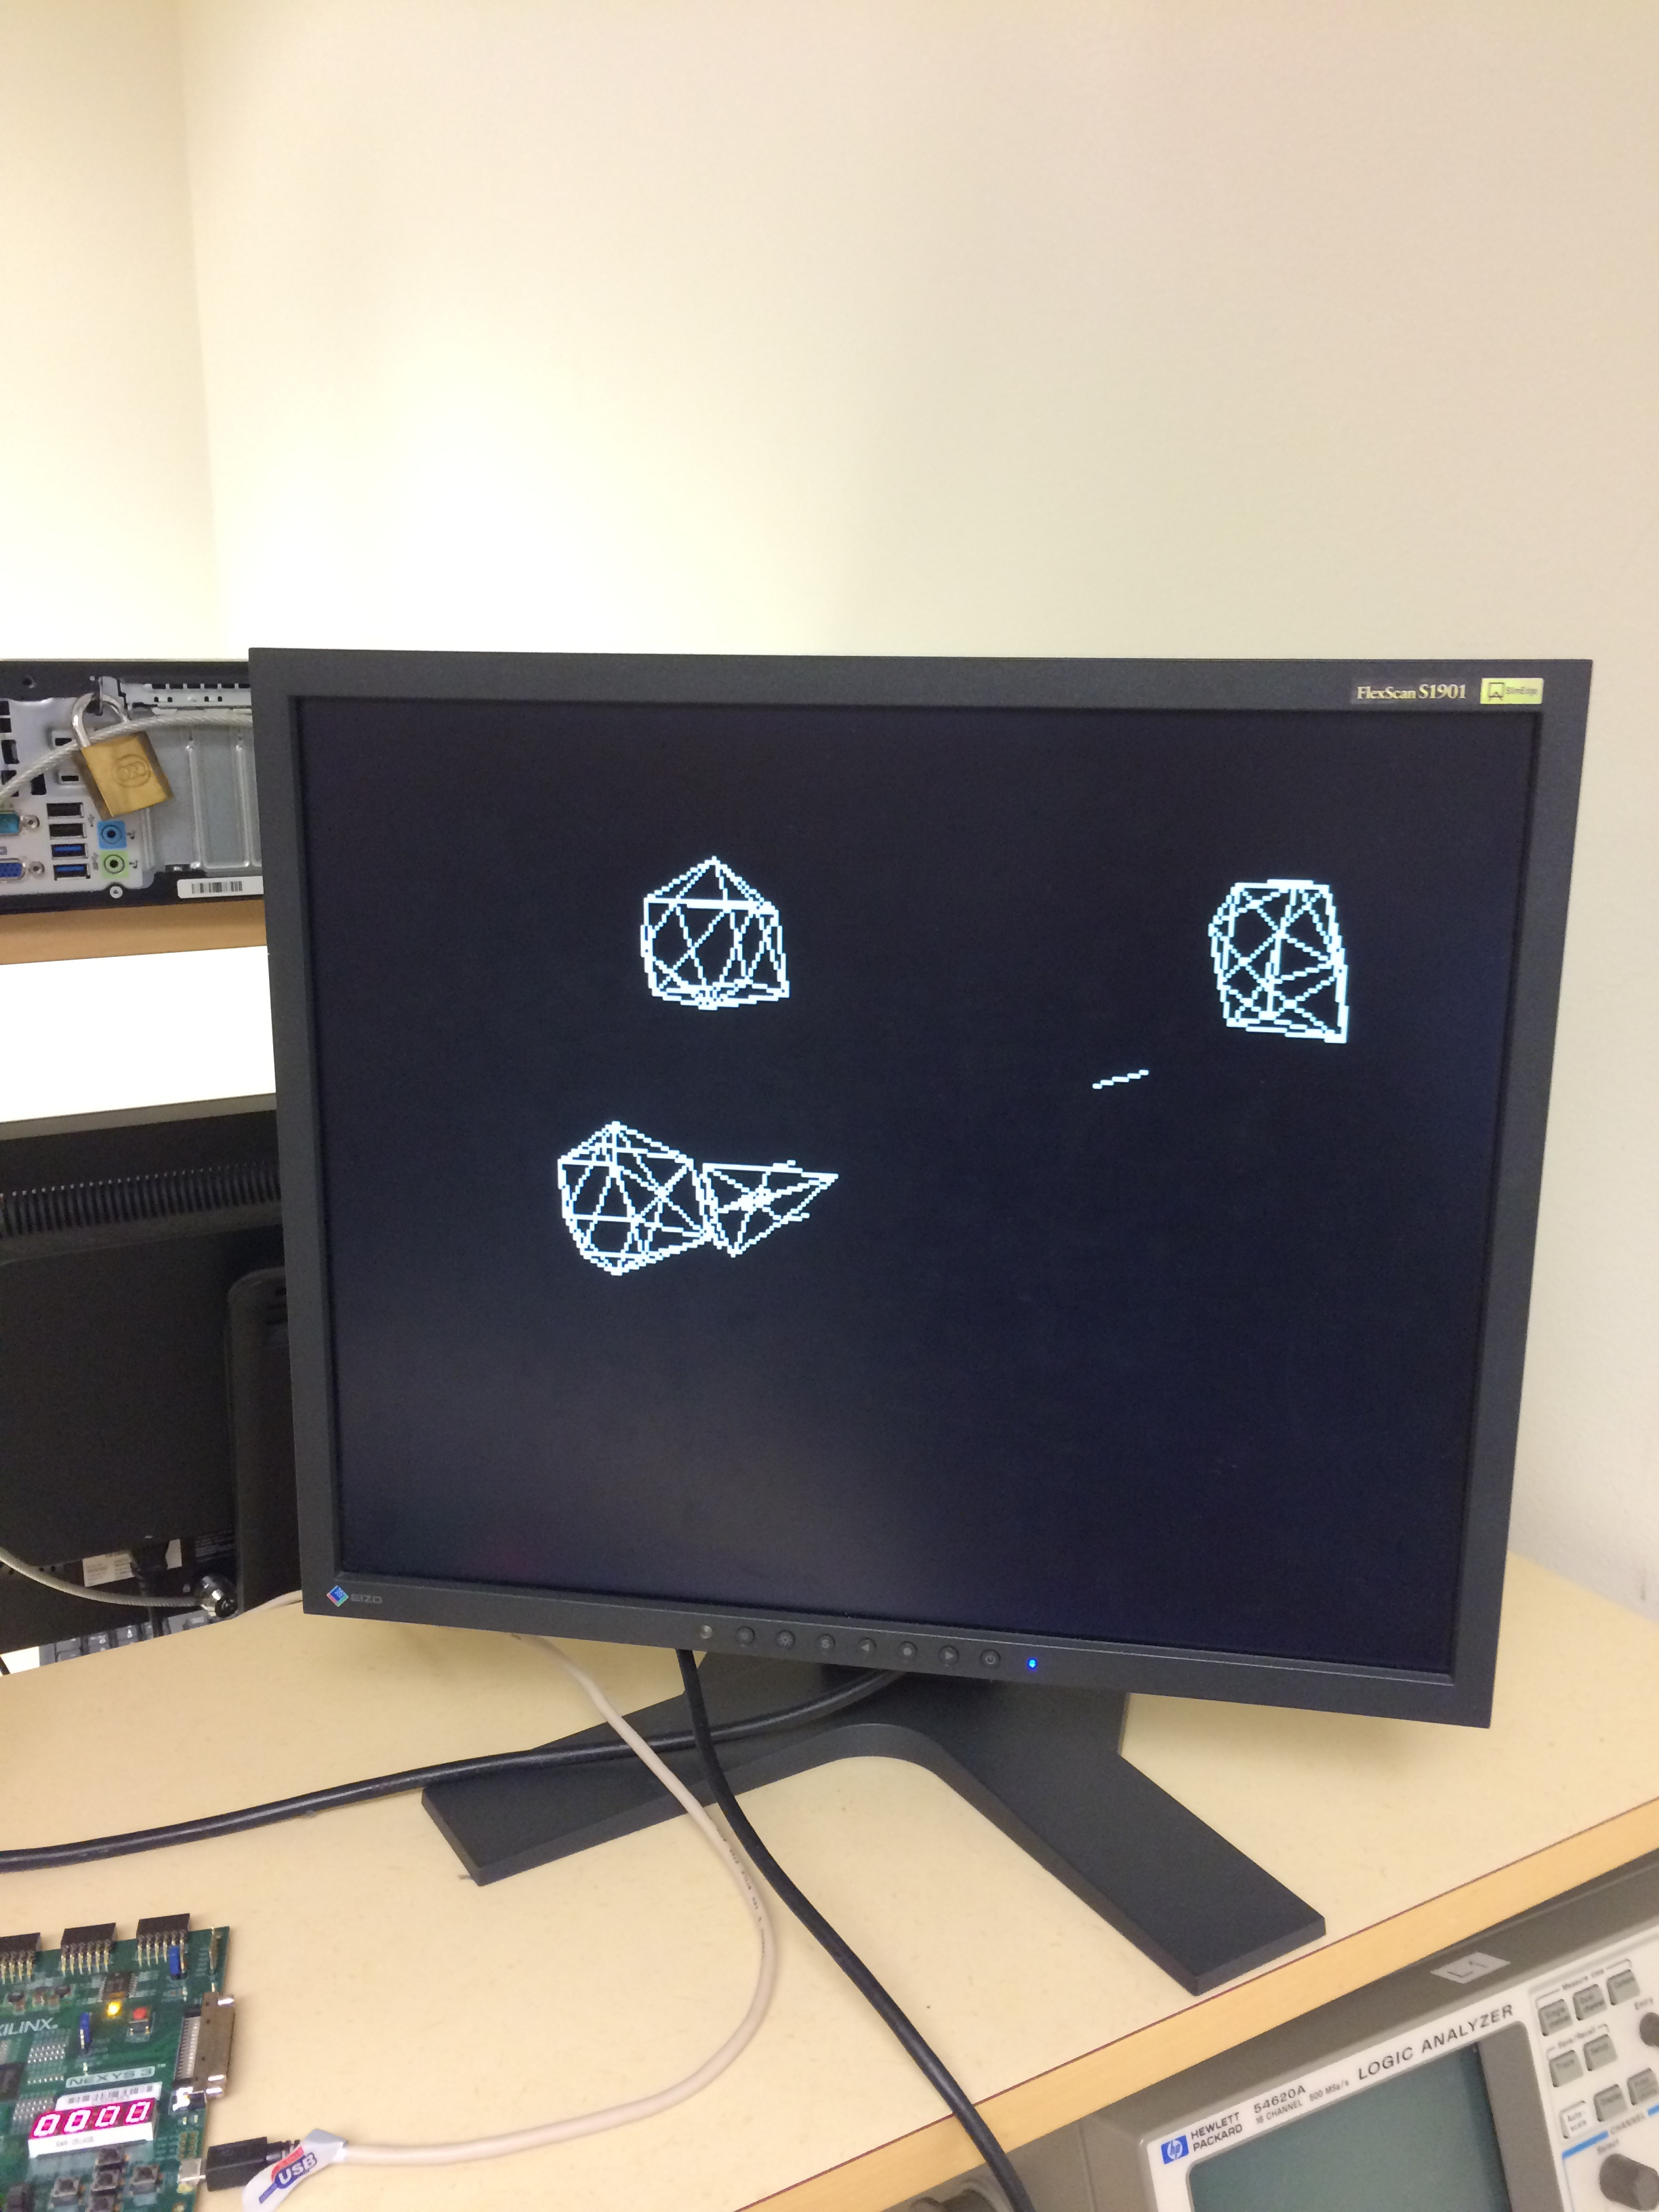
\includegraphics[width=0.7\textwidth]{title_img.jpeg} \par
    	{\huge\bfseries XYZ-Pilot\par}
        \vspace{1cm}
        \large{Jesper Westell, Patrik Sletmo \& Frans Skarman}

    	\vfill

        \large{\today}
    \end{titlepage}

    \tableofcontents
    \newpage
    
    \section{Inledning}
    Den här tekniska rapporten behandlar ett projektarbete i kursen TSEA83:
    Datorkonstruktion på Linköpings Universitet.





    \subsection{Bakgrund}
    Kursen TSEA83 läses av studenter på civilingenjörsprogrammet datateknik och
    avser att ge studenter kunskap om hur datorer fungerar i dess minsta
    beståndsdelar. Förutom projektarbetet består kursen av en förberedande
    laborationsdel som behandlar de grundläggande kunskaperna i
    processorkonstruktion och VHDL-kod\footnote{Kursplan för TSEA83 Datorkonstruktion, 
    studiehandboken på LiTH, \url{http://kdb-5.liu.se/liu/lith/studiehandboken/svkursplan.lasso?&k_kurskod=TSEA83&k_budget_year=2016}
    (hämtad 2016-05-24)}.
    


    \subsection{Syfte}
    Denna rapport syftar att ge en förståelse för vår konstruktions arkitektur
    och tekniska detaljer samt vilka lösningar vi tillämpat för att nå vår
    färdiga produkt. Läsaren ska efter att ha tagit del av rapporten ha
    förståelse för apparatens olika komponenter och de grundläggande teorier som
    krävs för detta. Rapporten förklarar också hur apparaten används för att
    fungera.


    \subsection{Källor}
    Det är en stor del av den här rapporten som bygger på i vanliga fall tveksamma källor, däribland
    diverse bloggposter och artiklar på Wikipedia. För en vanlig rapport hade det här inte varit
    acceptabelt utan rapporten borde istället hänvisat till mer seriösa källor för att verifiera att
    informationen stämde. I och med att den information som hämtats från utomstående källor är
    överrepresenterad av algoritmer och blockscheman tar den här rapporten inte det kravet på lika
    stort allvar.

    Överlag håller de källor som historisk fakta hämtats ifrån hög kvalité medan det
    snarare är representationer av algoritmerna som fallerar. I många fall har psuedokoden för en
    algoritm uppdaterats men inte dess förklaring vilket resulterar i viss förvirring när källorna
    ska tolkas.
    
    \newpage
        
    \section{Apparaten}
    Vår apparat använder ett tangentbord för input och visar sedan spelet på en
    skärm med hjälp av VGA. Programkoden, som innehåller instruktioner för
    processorn, laddas in via UART. Det program vi valt att realisera för apparaten
    är ett rymdspel som går ut på att skjuta sönder asteroider för poäng. Poängen
    man får syns hexadecimalt på 7-segments-displayen. Figur \ref{demo_img} visar en bild som
    beskriver hur konstruktionen ser ut.

    \begin{figure}[H]
        \centering
        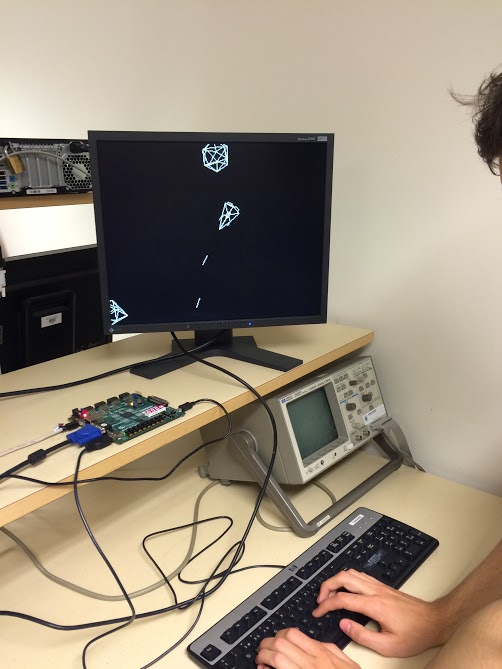
\includegraphics[width=0.8\textwidth]{demo_img}
        \caption{Med hjälp av tangentbordet är det möjligt att styra skeppet på
        skärmen och skjuta asteroider\label{demo_img}}
    \end{figure}
	
	\subsection{Användarhandledning}
    Konstruktionen byggs genom att koppla in VGA från skärmen, UART och
    strömsladd från valfri USB-port på en dator samt en tangentbordssladd i
    FPGAn enligt figur \ref{fig:connection}. För att starta programmet behöver du vara inne i
    mappen XYZ-Pilot/assembler och skriva in kommandot:
    
    \begin{lstlisting}[language=bash]
    ./assemble.sh game.asm
    \end{lstlisting}
 
    Detta skript programmerar hårdvaran och laddar in mjukvaran via UART. Inom
    kort borde skeppet synas på skärmen och tangentbordet kan användas för att
    spela. 

    \begin{figure}[H]
        \centering
        \includegraphics[width=0.8\linewidth]{connection.png}
        \caption{Bilden beskriver  de sladdar som ska kopplas in i kortet}
        \label{fig:connection}
    \end{figure}

    


    \section{Teori}
    \subsection{3D-grafik}
    3D-objekt representeras oftast som en mängd vektorer som beskriver hörnpunkter i
    objektet, linjer som binder ihop dessa vektorer och ytor som binder ihop dessa
    linjer. I vårt projekt finns inga ytor och för enkelhetens skull beskriver vi
    inte linjer som två index till punkter utan direkt som två vektorer. 

    I moderna GPUer används 4-dimensionella  vektorer istället för 3D vilket
    möjliggör rotation, skalning och translation av en vektor i en enda
    matrismultiplikation. Från början tänkte vi också göra det vilket är anledningen
    till att våra  vektorer är 4-dimensionella. 

    
    \subsection{Bresenhams linjealgoritm}
    Bresenhams linjealgoritm utvecklades på IBM under tidigt 1960-tal och hade den
    stora fördelen att dess implementation endast kräver heltalsaddition,
    subtraktion och shiftande av bitar. Eftersom algoritmen är så pass snabb och
    simpel finns den realiserad i många existerande grafikprocessorer och är
    anledningen varför vi valt att använda den i vårt projekt.  

    Algoritmen bygger på att räkna ut felet som uppstår jämfört motstående axel när
    algoritmen rör sig från början till slut. Blir felet tillräckligt stort
    korrigeras det och felet minskar då med en enhet. Felet ökar med absolutvärdet
    av kvoten mellan komponenternas längd för varje passerad pixel i algoritmens
    ursprungliga form, som då kräver decimaltalsaritmetik\footnote{Bresenham's Line Algorithm, \url{https://en.wikipedia.org/wiki/Bresenham\%27s_line_algorithm} (hämtad 2016-05-24)}. En implementation av
    detta följer nedan. 

    \begin{lstlisting}[]
func drawLine(x0, y0, x1, y1)
    dx = x1 - x0
    dy = y1 - y0
    e = -1
    de = abs(dy / dx)

    x = x0
    y = y0

    while x < x1 do
        fill(x, y)
        e += de
        if e >= 0 then
            y += 1
            e -= 1
        endif
        x += 1
    endwhile
endfunc
    \end{lstlisting}

    I och med att det är mer kostsamt och ineffektivt att använda
    decimaltalsaritmetik än heltalsaritmetik var en viktig egenskap med just
    Bresenhams algoritm att den går att skriva om för detta. En annan begränsning
    med algoritmen i dess grundutförande är att den endast fungerar för linjer som
    rör sig med riktningen av den sista oktanten och därför ser den algoritm som är
    implementerad i vår hårdvara aningen mer komplicerad ut än grundfallet. Vad som
    sker i hårdvaran går att göra enklare genom att använda transformering av in-
    och utdata beroende på vilken oktant linjen rör sig i istället för att använda
    if-satser. 

    \begin{lstlisting}[]
func drawLine(x0, y0, x1, y1)
    dx = abs(x1 - x0)
    dy = abs(y1 - y0)
    x = 0
    y = 0
    i = 0

    x_incr = 1 if (x1 - x0) > 0 else -1
    y_incr = 1 if (y1 - y0) > 0 else -1
    
    if dx > dy then
        len = dx
        D = 2 * dy - dx
    else
        len = dy
        D = 2 * dx - dy
    endif

    while i < len do
        fill(x, y)
        if D > 0 then
            if dx > dy then
                y += y_incr
                D -= 2 * dx
            else
                x += x_incr
                D -= 2 * dy
            endif
        endif
        
        if dx > dy then
            x += x_incr
            D += 2 * dy
        else
            y += y_incr
            D += 2 * dx
        endif

        i += 1
    endwhile
    
    fill(x, y)
endfunc
    \end{lstlisting}
    
    \subsection{Linear-Feedback Shift Register}
    För att implementera en slumpfunktion för vår apparat använder vi oss av ett så kallad 
    Linear-Feedback Shift Register, härmed kallad LFSR. Ett LFSR är ett register som med hjälp av 
    en inshiftad feedback-bit cyklar igenom ett antal tillstånd och på så sätt skapar en markant
    bättre slumpfunktion än att bara stega upp ett värde varje cykel. Genom att uppfylla ett visst
    antal faktorer går det att skapa en konfiguration för LFSR som resulterar i en maximal period.
    En maximal period innehåller $2^{antal\_bitar} - 1$ cykler innan värdet på registret upprepas.

    Ett LFSR bygger på att ett antal bitar av registret slås ihop med hjälp av en XOR-krets och
    sedan skiftas in som den mest signifikanta biten. Genom att välja ett register med jämt antal 
    relativt prima bitar som används i XOR-kretsen skapar man förutsättningen för att uppnå en
    optimal period för registret. För att underlätta skapandet av optimala LFSR används tabeller
    där de bitar som används för att skapa en maximal period är angivna. Eftersom komponenterna som
    används för att realisera kretsen endast bygger på XOR-grindar blir kretsen billig att tillverka
    och erbjuder ett stort värde jämfört med dess kostnad. Den funktion och det seed som används i
    vår apparat med 64-bitars register är illustrerat i nedanstående kodblock.

    \begin{lstlisting}[]
SEED = 0x0408151623422760
register = SEED

foreach clock
    next = ((register >> 0) ^ (register >> 1) ^ (register >> 3) ^ (register >> 4)) & 1
    register = (register >> 1) | (next << 15)
endforeach
    \end{lstlisting}

\section{Hårdvaran}

    Vår konstruktion består i grunden av en hårdvaruaccelererad grafikprocessor
    	för 3-dimensionella objekt och modeller som utökas med en centralprocessor
    som kan manipulera objekten som renderas och även utföra aritmetik på tal
    och vektorer. Programmet som körs på apparaten programmeras vid start via
    UART. En översikt av konstruktionen ses i blockschemat i figur
    \ref{fig:top_module}. 

    \begin{figure}[H]
        \centering
        \includegraphics[width=0.8\linewidth]{top_module.png}
        \caption{Översiktligt blockschema över  konstruktionen}
        \label{fig:top_module}
    \end{figure}
    
    \subsection{Centralprocessor}
	För att manipulera det som ritas med hjälp av grafikenheten används en processor 
	som med hjälp av instruktioner i programminnet bestämmer de värden som finns i 
	objektminnet. Processorn, som är naivt pipelinad, läser av instruktioner från 
	programminnet och utför beräkningar som får spelet att uppdateras. Alla minnen 
	och register är 64 bitar breda för att vektorer ska få plats på en adress. 
	Ett översiktligt blockschema finns i Figur \ref{fig:cpu}.

	För att spara programminne används extra hårdvara som automatiskt kör tre NOPar 
	mellan varje instruktion. Denna krets ger även möjligheten för processorn att “vänta” 
	på att VGA-motorn ska rendera klart en bild. En av processorns instruktioner får 
	NOP-logiken att ständigt skapa NOPar i processorn, något som kommer att pågå tills 
	VGA-motorn skickar en signal när den har renderat en bild.

	Det sista registret bland registerfilerna används för att spara information om vilka 
	knappar på tangentbordet är nedtryckta. Varje gång det finns en instruktion i IM4 som 
	inte skriver till något register passar processorn på att uppdatera detta register 
	från det register som finns i tangentbordsavkodaren. Detta innebär att de nedtryckta 
	tangenterna ständigt hålls uppdaterade eftersom majoriteten av instruktionerna som körs 
	är NOPar.

	\begin{figure}[H]
        \centering
        \includegraphics[width=0.8\linewidth]{CPU.png}
        \caption{Överskådligt blockschema över kretsen}
        \label{fig:cpu}
    \end{figure}
	
	\subsubsection{Vektorinstruktioner}
	Förutom vanliga instruktioner har processorn även stöd för instruktioner som hanterar 
	vektorer. Bland annat används addition och subtraktion av vektorer, samt skalärprodukt 
	och vektorlängd. Detta är möjligt tack vare separata komponenter som används i ALUn. 
	Innan en vektor ska användas vid beräkning delas den först upp i element som sedan används 
	på olika sätt beroende på vilken instruktion som körs. När beräkningar är gjorde sätts 
	elementen ihop igen för en resulterande vektor. En enkel illustration i figur \ref{fig:vector_instr} beskriver 
	hur detta fungerar. Notera att hårdvara för att bestämma kvadratroten av ett tal krävs för beräkning av vektorlängd. 
	Algoritmen för denna vhdl-kod har tagits från vhdlguru.blogspot.se\footnote{A VHDL Function for finding SQUARE ROOT, \url{http://vhdlguru.blogspot.se/2010/03/vhdl-function-for-finding-square-root.html} (hämtad 2016-05-27)}.

    \begin{figure}[H]
        \centering
        \includegraphics[width=0.8\linewidth]{vector_instr.png}
        \caption{Illustration över hur vektorinstruktioner fungerar}
        \label{fig:vector_instr}
    \end{figure}

    \subsection{UART}
    För att snabbt och enkelt ladda in programkod i programminnet används UART.
    Eftersom varje instruktion i programminnet är 64 bitar lång krävs det alltså 8
    bytes för att ladda in en hel instruktion. Detta görs genom två olika
    skiftregister, ett 10-bitars skiftregister som innehåller de 10 senaste bitarna
    och ett 64-bitars skiftregister som innehåller de 8 senaste bytes som laddats
    in. När 8 bytes laddats in (en hel instruktion) i UART-komponenten laddas dessa
    in i programminnet samtidigt som minnets nuvarande adress adderas med ett.
    Allt detta styrs av en styrenhet bestående av tre räknare, en som räknar varje
    klockpuls för varje bit, en som räknar alla bitar för varje byte och en som
    räknar alla bitar för varje instruktion. När dessa räknare nått sitt maxvärde
    sätts respektive laddpulser (sp, lp, mp) som får skiftregistren och
    programminnet att uppdateras. Den sista “instruktionen” består enbart av ettor
    och får UART-komponenten att sluta arbeta. Figur \ref{fig:uart_block} visar ett enkelt blockschema
    som beskriver kretsen. 

    \begin{figure}[H]
        \centering
        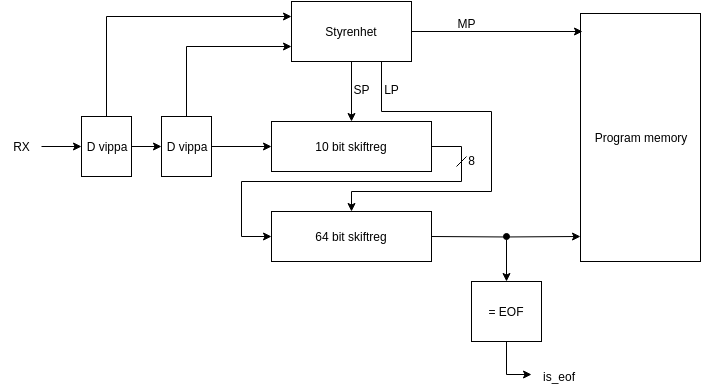
\includegraphics[width=0.8\linewidth]{uart_block}
        \caption{Blockschema för UART kretsen}
        \label{fig:uart_block}
    \end{figure}



    \subsection{Tangentbordsavkodare}

    För att använda ett tangentbord används en komponent som hanterar de
    PS/2-signaler som uppstår vid tangentnedtryck. Kretsen beskrivs i figur
    \ref{fig:kbd_dec}. En
    enkel tillståndsmaskin används för att ta reda på vilken tangent som är
    nedtryckt. Tillståndsmaskinen består av två tillstånd, IDLE och BREAK. Vid IDLE
    undersöks om nuvarande byte i shiftregistret stämmer med den kod för relevanta
    tangenter (--> tangenten sätts som nedtryckt) eller om koden är lika med den som
    föregår den sekvens som uppstår när en tangent släpps (--> tillståndet sätts till
    BREAK). Vid BREAK undersöks om nuvarande byte i shiftregistret stämmer med
    relevanta tangenter varvid tangenten sätts som uppsläppt. Tillståndet övergår
    alltid till IDLE vid BREAK.  

    \begin{figure}[H]
        \centering
        \includegraphics[width=0.8\linewidth]{kbd_dec}
        \caption{Blockschema för tangentbordsavkodaren}
        \label{fig:kbd_dec}
    \end{figure}

    \subsection{Objektminne}

    För att rendera modellerna på skärmen lagras olika objekt med specificerad
    modell, position och rotation. Objekten i minnet kan manipuleras med hjälp av
    processorinstruktioner och på så sätt ändra dess antal och egenskaper. 

    Formatet består av 4 ord per objekt där varje ord representerar en egenskap av
    position, rotation, skala samt en pekare till modellminnet i denna ordning.
    Notera att egenskapen för skala inte används i den nuvarande implementationen av
    grafikprocessorn utan finns kvar för kompatibilitetsskäl. Efter alla objekt
    finns ett ord bestående av enbart höga bitar. Strukturen på objektminnet kan ses
    i figur \ref{fig:obj_mem_structure}. 

    \begin{figure}[H]
        \centering
        \includegraphics[]{obj_mem_structure}
        \caption{Objektminnets struktur}
        \label{fig:obj_mem_structure}
    \end{figure}

    \subsection{Modellminne}
    Inprogrammerat i apparatens FPGA finns de modeller som apparaten stödjer där dessa lagras som
    ett antal linjer i en 3-dimensionell rymd. För att lättare fylla detta minne finns det verktyg
    för att konvertera Wavefrontmodeller (*.obj) till det format som används i VHDL-koden. Med 
    hjälp av detta och tillräckligt mycket minne kan vår apparat även användas för att
    förhandsgranska godtyckliga modeller.

    Formatet består av ett jämt antal ord där en linje består av ett ord för start och ett för
    stopp. De 16 första bitarna i ett ord för antingen start eller stopp representerar x-positionen
    och de 16 följande bitarna representerar y-positionen. Efter alla linjer följer två ord med 
    alla bitar höga för att indikera modellens slut. Se figur \ref{fig:model_mem_structure}.

    \begin{figure}[H]
        \centering
        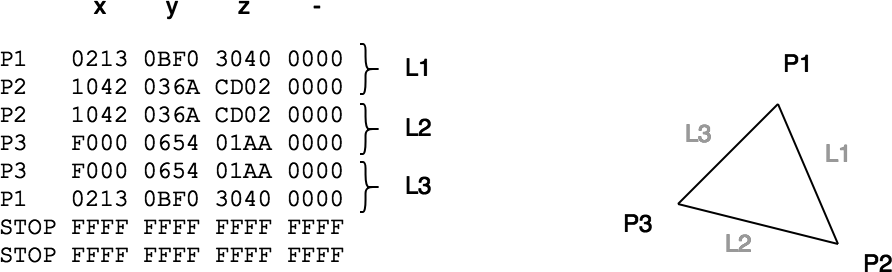
\includegraphics[width=0.8\linewidth]{model_mem_structure}
        \caption{Modellminnets struktur}
        \label{fig:model_mem_structure}
    \end{figure}

    \subsection{Grafikprocessor}
    Alla objekt definierade i objektminnet renderas varje bildskärmsuppdatering från
    dess 3-dimensionella representation till 2-dimensionella koordinater på skärmen
    med hjälp av apparatens grafikprocessor. Detta sker i ett antal steg som kan ses
    i figur \ref{fig:gpu_states}. 
    Grafikprocessorn kommer, 60 gånger i sekunden, läsa in alla objekt i
    objektminnet och omvandla deras information till pixelminnet. Vid uppdatering av
    ett objekt kommer grafikprocessorn först läsa in den information som finns i
    objektminnet. Därefter räknas trigonometriska värden ut från objektets rotation.
    Nu kommer grafikenheten, för varje linje i objektets modell, bestämma vilka
    pixlar mellan start- och slutpunkt som ska sättas som “vit” i pixelminnet. 

    \begin{figure}[H]
        \centering
        \includegraphics[width=0.8\linewidth]{gpu_states}
        \caption{Översiktligt state-diagram för GPUn}
        \label{fig:gpu_states}
    \end{figure}

    \subsubsection{Inläsning av modeller}
    Varje linje i en modell består av två vektorer, en start och en slutvektor. Dessa står i
    modellminnet och en modell avslutas med en linje som har enbart höga bitar som både start
    och slutvektor. Om den inlästa inte är en slutmarkör går GPUn vidare till nästa
    state, annars går den till att läsa nästa modell. (egentligen sker den kollen
    efter beräkningen av den roterade vektorn). 

    \subsubsection{Beräkning av trigonometriska funktioner}
    Objektets rotation används för att beräkna olika trigonometriska värden som
    används i beräkningen av linjernas koordinater med avseende på rotationen. Det
    sker med hjälp av ett "sinus lookup table" där varje kombination av sin och cos
    för x,y,z vinkeln beräknas sekventiellt. 

    \subsubsection{Beräkning av linjens roterade position}
    Den nyligen inlästa linjen roteras med hjälp av en rotationsmatris (figur
    \ref{fig:rot_matrix}) som beräknas med de värden som tidigare bestämdes för
    objektets rotation. Egentligen beräknas inte rotationsmatrisen utan
    resultatet av rotationsmatrisen multiplicerat med positions vektorn beräknas
    direkt. Eftersom GPUn inte hanterar djup beräknas bara X och  Y
    elementen i den nya positionen. Den roterade vektorn kan ses i
    figur \ref{fig:rotated_vector}. 

    \begin{figure}
        \[
            \begin{pmatrix}
                cos(c) & -sin(c) & 0 \\ 
                sin(c) & cos(c)  & 0 \\
                0      &    0    & 1
            \end{pmatrix}
            \cdot
            \begin{pmatrix}
                cos(c)  &    0    & sin(b) \\ 
                0       &    1    & 0 \\
                0       &    0    & cos(b)
            \end{pmatrix}
            \cdot
            \begin{pmatrix}
                cos(b) & 0 & sin(b) \\ 
                0 & 1  & 0 \\
                -sin(b)      &    0    & cos(b) \\
            \end{pmatrix}
            \cdot
            \begin{pmatrix}
                x \\
                y \\
                z \\
            \end{pmatrix}
        \]
        \caption{Matriserna som ska multipliceras för att rotera med eulervinklar \((a, b, c)\)}
        \label{fig:rot_matrix}
    \end{figure}

    \begin{figure}
        \[
            \begin{pmatrix}
x cos(b) cos(c)+y (cos(c) sin(a) sin(b)-cos(a) sin(c))+z (cos(a) cos(c) sin(b)+sin(a) sin(c)) \\
x cos(b) sin(c)+z (cos(a) sin(b) sin(c)-cos(c) sin(a))+y (cos(a) cos(c)+sin(a) sin(b) sin(c)) \\
z cos(a) cos(b)+y sin(a) cos(b)-x sin(b)
            \end{pmatrix}
        \]
        \caption{Resultatet vid matrismultiplikation}
        \label{fig:rotated_vector}
    \end{figure}

    Beräkningen sker sekventiellt för både start och slutvektorn för linen. För
    att beräkna varje element beräknas först de trigonometriska funktionerna
    ihop två och två. Är det exempelvis tre trigonometriska funktioner i en delberäkning sparas
    resultatet av de två första i en buffer som sedan multipliceras med den
    tredje. När en delberäkning är klar multipliceras den med ett av elementen
    i positionsvektorn och resultatet sparas i en accumulator. När ett helt
    element i slutvektorn har beräknats sparas det och nästa element beräknas.
    När processen är klar för både start och slutvektorn går GPUn vidare till
    att rita ut linjerna. Ett blockschema för processen kan ses i figur
    \ref{fig:rotation_hardware} 

    \begin{figure}[H]
        \centering
        \includegraphics[width=0.7\linewidth]{rotation_hardware}
        \caption{Blockschema över hårdvaran som utför rotation av vektorer}
        \label{fig:rotation_hardware}
    \end{figure}

    \subsubsection{Utritning av linje}
    När linjens början och slut bestämts i skärmkoordinater används Bresenhams
    linjealgortim för att rita ut den. Först förbereds algortimens
    begynnelsevillkor för att sedan stega igenom den axel för linjen som är
    längst och fylla de positioner som stegas igenom i pixelminnet. En
    detaljerad beskrivning av algoritmen finns i teorikapitlet.

    \subsubsection{Väntan}

    När alla objekt ritats ut väntar grafikprocessorn med att börja om
    utritningen tills vga-motorn signalerat att en bild skickats till
    bildskärmen. 

    \subsection{Pixelminne}

    Pixelminnet fungerar som kommunikationsbrygga mellan GPUn och VGA-motorn.
    Eftersom GPUn inte kommer ihåg vilka linjer som har ritats ut så måste
    skärmen någon gång rensas från den förra bilden. Vi valde att låta VGA motorn
    sköta det eftersom att den ändå stegar igenom varje pixel i bilden. Ett problem
    med den lösningen är att GPUn inte kan rita sin bild samtidigt som VGA motorn
    rensar då delar av bilden i så fall skulle rensas bort innan de ritas ut. Därför är
    pixelminnet dubbelbuffrat. 

    Pixelminnet består alltså av två identiska block-RAM, ett som GPUn skriver till och ett
    som VGA-motorn läser från och rensar. När VGA-motorn är färdig med en bild signalerar
    den till pixelminnet att det ska byta RAM som läses och skrivs. Då läser VGA-motorn 
    från det RAM som GPUn skrev till vid förra bilduppdateringen och GPUn får
    ett nyrensat minne att skriva i. 

    \begin{figure}[H]
        \centering
        \includegraphics[width=0.8\linewidth]{pixelmem}
        \caption{Blockschema över pixelminnet}
        \label{fig:pixelmem}
    \end{figure}

    \subsection{VGA motorn}

    VGA-motorn är den komponent som stegar igenom varje pixel på skärmen för att
    sätta ett bildvärde på dem. En pixel kan vara svart eller vit. Denna
    information fås från pixelminnet som VGA-motorn har konstant kommunikation
    med. Eftersom det tar en klockpuls för att läsa från pixelminnet bestämmer
    VGA-motorn vilken position på skärmen som den borde vara vid nästa klockpuls
    för att synka positionen på skärmen med det värde som fås från pixelminnet.
    Bilden som ritas ut är 320x240 som skalas upp till 640x480. Detta innebär
    att varje “storpixel” i pixelminnet beskriver vilken färg som 4 pixlar på
    skärmen ska få. För att få ut rätt adress i pixelminnet vid läsning
    divideras x- och y-position enkelt med 2. När den sista pixeln för en
    “storpixel” sätts på skärmen skickar VGA-motorn en signal till pixelminnet
    för att nollställa just den “storpixeln”. När en hel bild har uppdaterats
    sänds en signal till konstruktionens CPU och GPU för att informera att de
    ska fortsätta jobba. En detaljerad beskrivning syns i figur \ref{fig:VGA_motor}. 

    \begin{figure}[H]
        \centering
        \includegraphics[width=0.8\linewidth]{VGA_motor}
        \caption{Blockschema över VGA motorn}
        \label{fig:VGA_motor}
    \end{figure}

    \subsection{Matematikhårdvara}
    För att rita 3D-modeller fanns två stora matematiska problem som behövde
    lösas. För det första behövdes hårdvara för att behandla vektorer som
    används för den största delen av 3D-grafiken och spellogiken. Det andra som
    behövdes är hårdvara för beräkning av sinus- och cosinus-värden för vinklar som
    används vid rotation.
    
    \subsubsection{Vektorer}
    Hårdvaran för att behandla vektorer har två viktiga jobb, att spara vektorer
    och att göra matematiska beräkningar på dem. Vektorer sparas som vanliga
    bitvektorer i datorns minne där varje 16 bitar representerar ett element i
    vektorn och vi har en komponent som kan gå från minnesrepresentation till
    element och en som kan gå tvärt om. 

    Vektor-addition och subtraktion är relativt enkla, kombinatoriska kretsar
    adderar och
    subtraherar bara varje element i vektorn. Även skalärprodukt och
    längdberäkningarna görs kombinatoriskt precis som det skulle göras rent
    matematiskt. 

    \subsubsection{Trigonometriska funktioner}
    För att "beräkna" cosinus- och sinus-värden av vinklar används ett enkelt lookup
    table som tar en 8 bitars vinkel och returnerar ett värde för cosinus eller
    sinus. För att förenkla hårdvaran beräknas sinus i CPUn genom att addera en
    fjärdedels period till vinkeln och beräkna cosinus av den vinkeln. 

    \subsubsection{Beräkningar med "små" tal}
    Eftersom att VHDL inte har inbyggt stöd för varken flyttal eller någon form
    av fixed point system behövde vi designa ett eget system för att
    multiplicera tal som är mindre än 1. Grundprincipen är att vi väljer en
    plats i bitvektorn där heltals delen börjar. Alla heltal förskjuts så att de
    börjar vid den punkten, sedan multipliceras talen med varandra och förskjuts
    tillbaka dubbelt så långt. Detta fungerar tack vare ekvation
    \ref{eq:mult_shift}

    \begin{equation}
        \label{eq:mult_shift}
        a \cdot b = \frac{a 2^n}{2^n} \cdot \frac{b 2^n}{2^n} = \frac{a2^n *
        b2^n}{2^{2n}}
    \end{equation}

    Eftersom vi inte var säkra på hur aritmetiska shift-funktoner skulle
    behandla signed tal valde vi att implementera ett eget format för små tal.
    Vi insåg att vi aldrig skulle behöva multiplicera två stora tal med varandra
    och bry oss om decimal delen, det räcker med multiplikation av små
    "decimaltal" och multiplikation av heltal med små decimaltal. De stora talen
    behandlas endast som 16 bitars signed tal samtidigt som små tal är 16 bitars
    bitvektorer där den sista biten är sign-bit och de 9 första bitarna är
    storleken på talet, sparad som unsigned där bit nummer 9 är den enda heltals-biten
    för att möjliggöra sparning av talet 1. 

    Multiplikation av två små tal sker genom att de två "storleksdelarna"
    multipliceras ihop och resultatet förskjuts tillbaka åt höger. Tecknet på
    det nya talet blir XOR av de två original tecknen. Ett blockschema för
    kretsen kan ses i figur \ref{fig:small_numbers}.

    Multiplikation av ett litet och ett stort tal är aningen mer komplicerat
    eftersom det stora talet är signed och resultatet också ska vara ett
    signed tal. Absolutbeloppet av det stora talet förskjuts 8 bitar åt vänster
    och multipliceras med värdes delen av det lilla talet. Resultatet förskjuts
    tillbaka 16 bitar. För att få rätt tecken på resultatet multipliceras
    resultatet med -1 om xor av de båda talens teckenbit är 1. Även den här
    processen beskrivs i figur \ref{fig:small_numbers}.


    \section{Mjukvara}
    \subsection{Assembler}

    För att lättare kunna skapa program till apparaten har vi designat ett program
    för att tolka assemblykod och konvertera det till maskinkod som sen kan laddas
    in via UART och exekveras. Genom att också förse assemblern med vissa mer
    avancerade programstatser blir det väldigt enkelt att skapa större program. 

    \subsubsection{Labels}
    En av de enklaste funktionerna i en assembler är att kunna namnge hoppadresser
    och på så sätt slippa ändra hoppadresser varje gång som kod läggs till i mitten
    av programmet. 

    \subsubsection{Variabler}
    Det är möjligt att definiera variabler längst med programmet som det
    reserveras en minnesplats till i arbetsminnet. Variabler kan antingen
    användas som konstanter eller ändras allt eftersom med hjälp av samma
    syntax. 
    \subsubsection{Registeralias}
    Eftersom variabler endast kan användas i instruktionerna LOAD och STORE blir
    det många instruktioner som använder så kallade magiska nummer för att
    referera till de register som används. Lösningen som används i vår assembler
    stödjer därför möjligheten att sätta alias för register. Genom att också
    uppdatera dessa alias så fort man laddar in ett värde med LOAD blir
    programstrukturen betydligt mer lättöverskådlig. 
    \subsubsection{Kommentarer}
    På grund av begränsningar i tolkens funktionalitet kan bara en typ av
    statement användas per rad, och det gäller även för kommenterar. Rader som
    börjar med tecknet för kommentarer hamnar inte i den genererande
    programkoden och kan istället användas för att förklara koden. 
    \subsubsection{Loopar}
    Eftersom mycket i det program som används för apparaten bygger på att iterera över diverse data
    blir det lätt krångligt att hålla koll på alla labels som behövs. För att göra programflödet
    tydligare i utvecklingsfasen innehåller därför assemblern stöd för att upprepa en mängd kod
    tills dess villkor inte längre är uppfyllt. Assemblern genererar automatiskt kod för att ladda
    in eventuella variabler i register och kan även operera direkt på registeralias.

    \begin{lstlisting}
WHILE X >= Y
    # Perform operation
ENDWHILE
    \end{lstlisting}

    \subsubsection{Villkorligt programflöde}
    För att utöka syntaxen för programflödet ytterligare erbjuder assemblern möjligheten att
    deklarera villkorligt programflöde, även kallat if-satser. Rent funktionellt är det mycket som
    denna syntax har gemensamt med looparna, båda läser in och jämför variabler och registeralias på
    samma sätt. Skillnaden är att if-satser endast kollar villkoret en gång och går sedan vidare.
    En begränsning med denna sats är att den endast stödjer en jämförelse i taget, det går alltså
    inte att ändra flödet ifall två villkor eller minst ett av flera villkor stämmer. För att uppnå
    den funktionaliteten behöver man kedja flera satser för att uppnå önskat resultat. Det finns
    heller inget stöd för att agera på motsatsen till ett villkor.

    \begin{lstlisting}
IF X == Y
    # Operation 1
ENDIF
IF X != Y
    # Operation 2
ENDIF
    \end{lstlisting}

    \subsection{3D modeller}
    3D-modeller kan skapas i valfritt 3D-modellerings program som kan exporteras
    till .obj-format. Med hjälp av två skript kan .obj-filen sedan konverteras
    till data som läggs in i modellminnet. Det första skriptet,
    obj\_converter.py
    konverterar en .obj-fil till koordinaterna för alla linjer i modellen. Det
    andra  skriptet, coord\_generator.py tar listan av koordinater och genererar
    data som passar i objektminnet. Det andra skriptet kan ta en parameter
    som bestämmer var i objektminnet modellen ska börja så man enkelt kan
    lägga till modellerna efter varandra. Hela operationen kan göras med
    följande kommando:

    \begin{lstlisting}[language=bash]
        python3 obj_converter.py <filnamn>.obj | python3 coord_converter <start index>
    \end{lstlisting}

    Resultatet av ovanstående kommando är en lång lista av minnesdata till
    modellminnet som ska läggas in i deklarationen av modellminnet.

    \subsection{Spellogiken}
	Spelet kan ses som en stor loop där allt i loopen sker 60 gånger i sekunden. Flödesschemat
	i figur \ref{fig:game_logic} visar en ungefärlig bild över hur spelet fungerar. Nytt spel
	startas alltid med att initialisera värden och sätta variabler. Efter detta hamnar kontrollflödet
	i den stora loopen som börjar med att uppdatera skeppets position. Precis innan skeppets slutgiltiga
	position skrivs i objektminnet görs en kontroll om skeppet är utanför någon gräns. Om detta 
	stämmer nollställs hastigheten i den riktningen och positionen justeras innan det
	skrivs in i objektminnet. Efter detta uppdateras skottens position och ett eventuellt nytt 
	skott skjuts iväg. Asteroiderna uppdateras i flera steg. Först kontrolleras det om någon asteroid 
	hamnat utanför en gräns som satts. Om detta stämmer ändras asteroidens position till en fast punkt,
    ASTEROID\_GRAVEYARD som det döpts till i koden. När denna kontroll gjorts för alla asteroider kommer 
	de att uppdatera sin position och rotation. De som nyligen flyttats till ASTEROID\_GRAVEYARD kommer 
	få en ny position utanför skärmen, slumpmässigt valt längs en rektangel utanför skärmen, samtidigt 
	som de får en slumpmässig hastighet och rotation. För varje asteroid kontrolleras även kollision
	med skott, varvid asteroidens position uppdateras till ASTEROID\_GRAVEYARD och antalet poäng ökas. 
	Slutligen kontrolleras kollision mellan skeppet och någon av asteroiderna. Om detta stämmer har 
	spelaren förlorat och spelet startas på nytt. Om ingen kollision skett kommer processorn vänta på att
	VGA-motorn renderat en skärm innan den gör om allt igen. Kollisionsdetektion sker genom att kolla 
	vektorlängden mellan två objekts postionsvektorer.
	
	\begin{figure}[H]
        \centering
        \includegraphics[width=0.8\linewidth]{game_logic.png}
        \caption{Flödesschema över spelets logik}
        \label{fig:game_logic}
    \end{figure}

	\section{Slutsatser}
        Med vår apparat har vi utvärderat flera olika tekniker och algoritmer som använts i verklig
        hårdvara. Vi kan med kunskapen vi funnit efter att ha implementerat dessa på egen hand
        konstatera att mycket tidig hårdvara hade hårda krav på simplicitet i kretsarna där både
        Bresenham's Linjealgoritm och Linear-Feedback Shift Register är tydliga exempel på detta. Vi
        visste i början av projektet att funktioner som liknade dessa skulle behövas men det var inte
        förrän vi började som vi tittade på de här historiska komponenterna på riktigt.

        Den större
        delen av vår grafikprocessor är väldigt mycket mer komplicerad än dessa kretsar och bygger
        på komplicerade trigonometriska kretsar. Trots att vi visste att det skulle innebära mycket
        matematik att implementera den tredimensionella projektion vi definierat i 
        designspecifikationen var vi inte beredda på riktigt hur mycket som skulle krävas, vilket är
        varför all planerad funktionalitet inte implementerats. Med detta sagt är det mycket vi
        lärt oss om grafikprocessorer i det här projektet som lyft det området inom datateknik för
        hela gruppen och det har blivit lättare att greppa vad ett grafikkort faktiskt gör.

        Grafikprocessorn är den del i projektet där vi haft minst tidigare erfarenhet eller
        dokumentation att gå på. I princip alla andra delar av apparaten har vi kunnat använda
        simpla och beprövade kretsar med inspiration från algoritmer och blockscheman. CPU:n som är
        den näst mest komplicerade kretsen i apparaten har vi fått förklarad under föreläsningar och
        laborationer så det har inte blivit särskilt mycket nytt att resonera runt där. GPU:n har
        beprövat våra kunskaper i VHDL och hårdvarutänkande i allt från design av blockscheman till
        att vara konsekvent i kodbasen. Hade det gått att implementera den här kretsen på ett bättre
        sätt än vi gjort? Ja, helt klart. Det finns många designfel i vår apparat ur ett
        hårdvaruperspektiv men det betyder inte att vi inte har en bra lösning; med den tidigare
        kunskap inom ämnet vi har är det orimligt att vänta sig att vi skulle upptäcka de felen från
        början. När projektet närmade sig sitt slut kunde vi identifiera vissa fel som ledde till
        sämre prestanda men eftersom vår apparats resurser låg långt över gränsen för vad som
        faktiskt behövdes och eftersom tiden var knaper valde vi att inte ta itu med problemen.

        I det stora hela har möjligheten att kunna definiera fullständigt godtyckliga logiska 
        kretsar med hjälp av VHDL inneburit att vi lärt oss otroligt mycket inom ämnet och det har
        i princip bara varit tiden och FPGA-chipets storlek som satt gränserna. Faktum är att vi
        med tillräckligt mycket tid säkert hade kunnat implementerat hela vår designspecifikation
        och även projicera det tredimensionella rummet med djup - trots att vi inte kunnat något
        alls om ämnet tidigare.

    \section{Referenser}
    \begin{enumerate}
      \item Bresenham's Line Algorithm, \url{https://en.wikipedia.org/wiki/Bresenham\%27s_line_algorithm} (hämtad 2016-05-24)
      \item Kursplan för TSEA83 Datorkonstruktion, 
        studiehandboken på LiTH, \url{http://kdb-5.liu.se/liu/lith/studiehandboken/svkursplan.lasso?&k_kurskod=TSEA83&k_budget_year=2016} (hämtad 2016-05-24)
      \item A VHDL Function for finding SQUARE ROOT, \url{http://vhdlguru.blogspot.se/2010/03/vhdl-function-for-finding-square-root.html} (hämtad 2016-05-27)
    \end{enumerate}

    \section{VHDL kod}
    Koden är väl kommenterad och borde vara lätt att förstå med hjälp av den här
    rapporten. En sak som kan vara värd att notera är dock att deklarationen av
    GPU\_Info som innehåller ett antal typdeklarationner som används i GPUn
    ligger i model\_mem.vhd. Detta är på grund av att vi hade problem med
    include ordningen i makefilen och inte har flyttat ut GPU\_Info igen.
\end{document}


%notes
\iffalse
\fi
